\chapter{Invariant mass fits to \decay{\Bp}{\Dsp\phiz} simulations}
\label{ch:appendix_MCfits}


%%%%%%%%%%%%%%%%%%%%%%%%%%%%%%%%%%%%%%%%%%%%%%%%%%%%%%%%%% 
\begin{table}[h]
   \centering
   \begin{tabular}{ c c c c }
      \hline
      \multirow{2}{*}{Parameter}                   & \multicolumn{3}{c} {Value} \\
      \cline{2-4}
                                  & \decay{\Dsp}{\Kp\Km\pip}   & \decay{\Dsp}{\Kp\pim\pip} & \decay{\Dsp}{\pip\pim\pip}  \\
      \hline
      %\textbf{$\B \to \Ds \phi$}  &                    &                    &                        \\
      \multicolumn{4}{l} {\decay{\Bp}{\Dsp\phiz}}\\

      \hline
      $\sigma_1/\sigma_2$         & 0.49 $\pm$ 0.01    & 0.47 $\pm$ 0.01    & 0.46 $\pm$ 0.01        \\
      $f_\sigma$                  & 0.80 $\pm$ 0.01    & 0.84 $\pm$ 0.01    & 0.81 $\pm$ 0.01        \\
      $\alpha$                    & 2.76 $\pm$ 0.07    & 3.06 $\pm$ 0.16    & 3.71 $\pm$ 0.23        \\
      $n$                         & 1 $\pm$ 0          & 1  $\pm$ 0         & 1  $\pm$ 0             \\
      \hline
      %\textbf{ }  &                    &                    &                        \\
      \multicolumn{4}{l} {\decay{\Bp}{\Dsp\Dzb}}\\
      \hline
      $\sigma_1/\sigma_2$         & 0.43 $\pm$ 0.01    & 0.42 $\pm$ 0.01    & 0.40 $\pm$ 0.01        \\
      $f_\sigma$                  & 0.88 $\pm$ 0.01    & 0.88 $\pm$ 0.01    & 0.88 $\pm$ 0.01        \\
      $\alpha$                    & 2.91 $\pm$ 0.06    & 3.36 $\pm$ 0.26    & 3.53 $\pm$ 0.25        \\
      $n$                         & 1 $\pm$ 0          & 1 $\pm$ 0          & 1 $\pm$ 0              \\
      \hline 
      $\sigma_{1}(\Dsp\phi) / \sigma_{1}(\Dsp\Dzb)$ & 1.27 $\pm$ 0.02 & 1.31 $\pm$ 0.02 & 1.26 $\pm$ 0.02 \\
      \hline
   \end{tabular}
   \caption{Fixed values obtained in fits to MC used in the model for the signal pdf.} 
   \label{tab:DsPhi_mc_fits}  
\end{table}
%%%%%%%%%%%%%%%%%%%%%%%%%%%%%%%%%%%%%%%%%%%%%%%%%%%%%%%%%% 


%%%%%%%%%%%%%%%%%%%%%%%%%%%%%%%%%%%%%%%%%%%%%%%%%%%%%%%%%%
\begin{figure}[!h]
   \centering
   \begin{subfigure}[t]{1.0\textwidth}
      \centering
      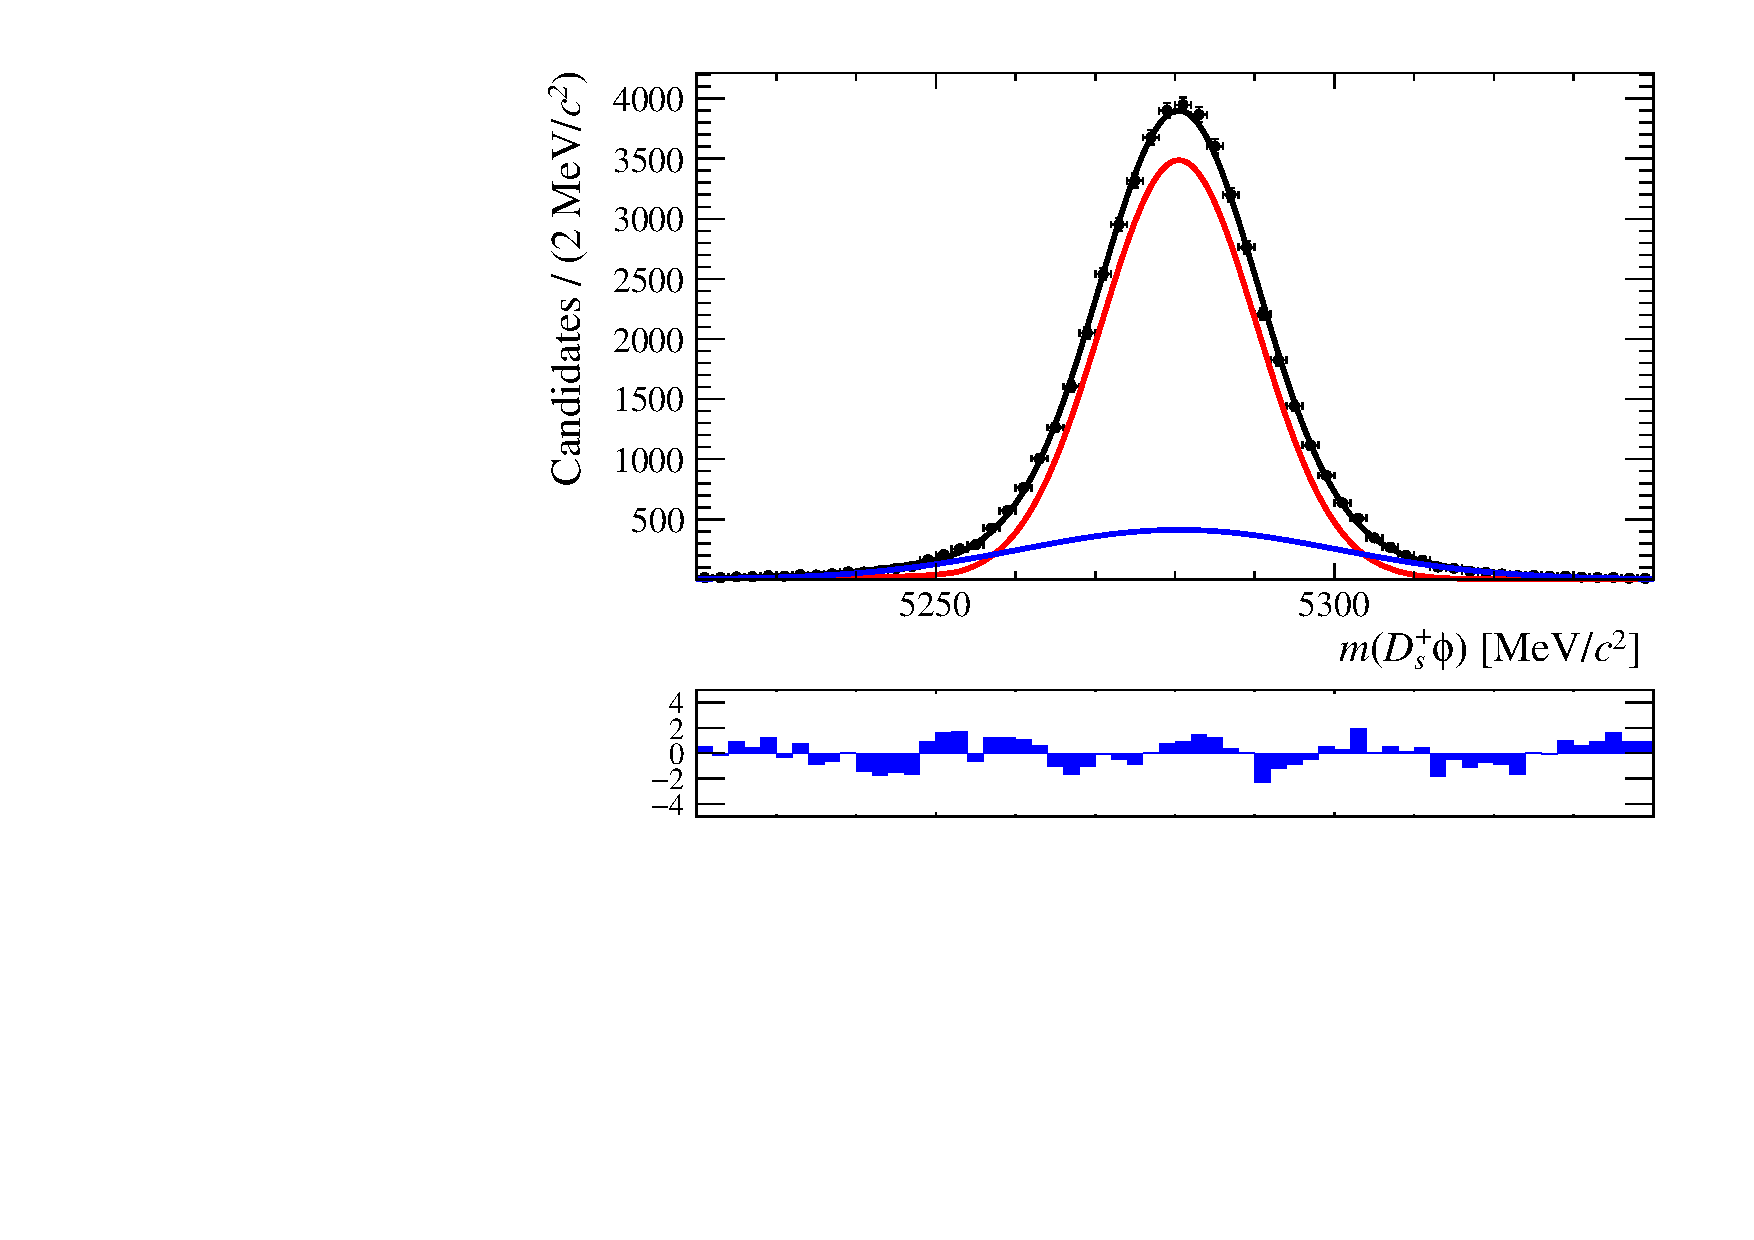
\includegraphics[width=0.40\textwidth]{figs/B2DsPhi/Plot_Signal_Fit_All_B2PhiDs_Ds2KKPi.pdf}
      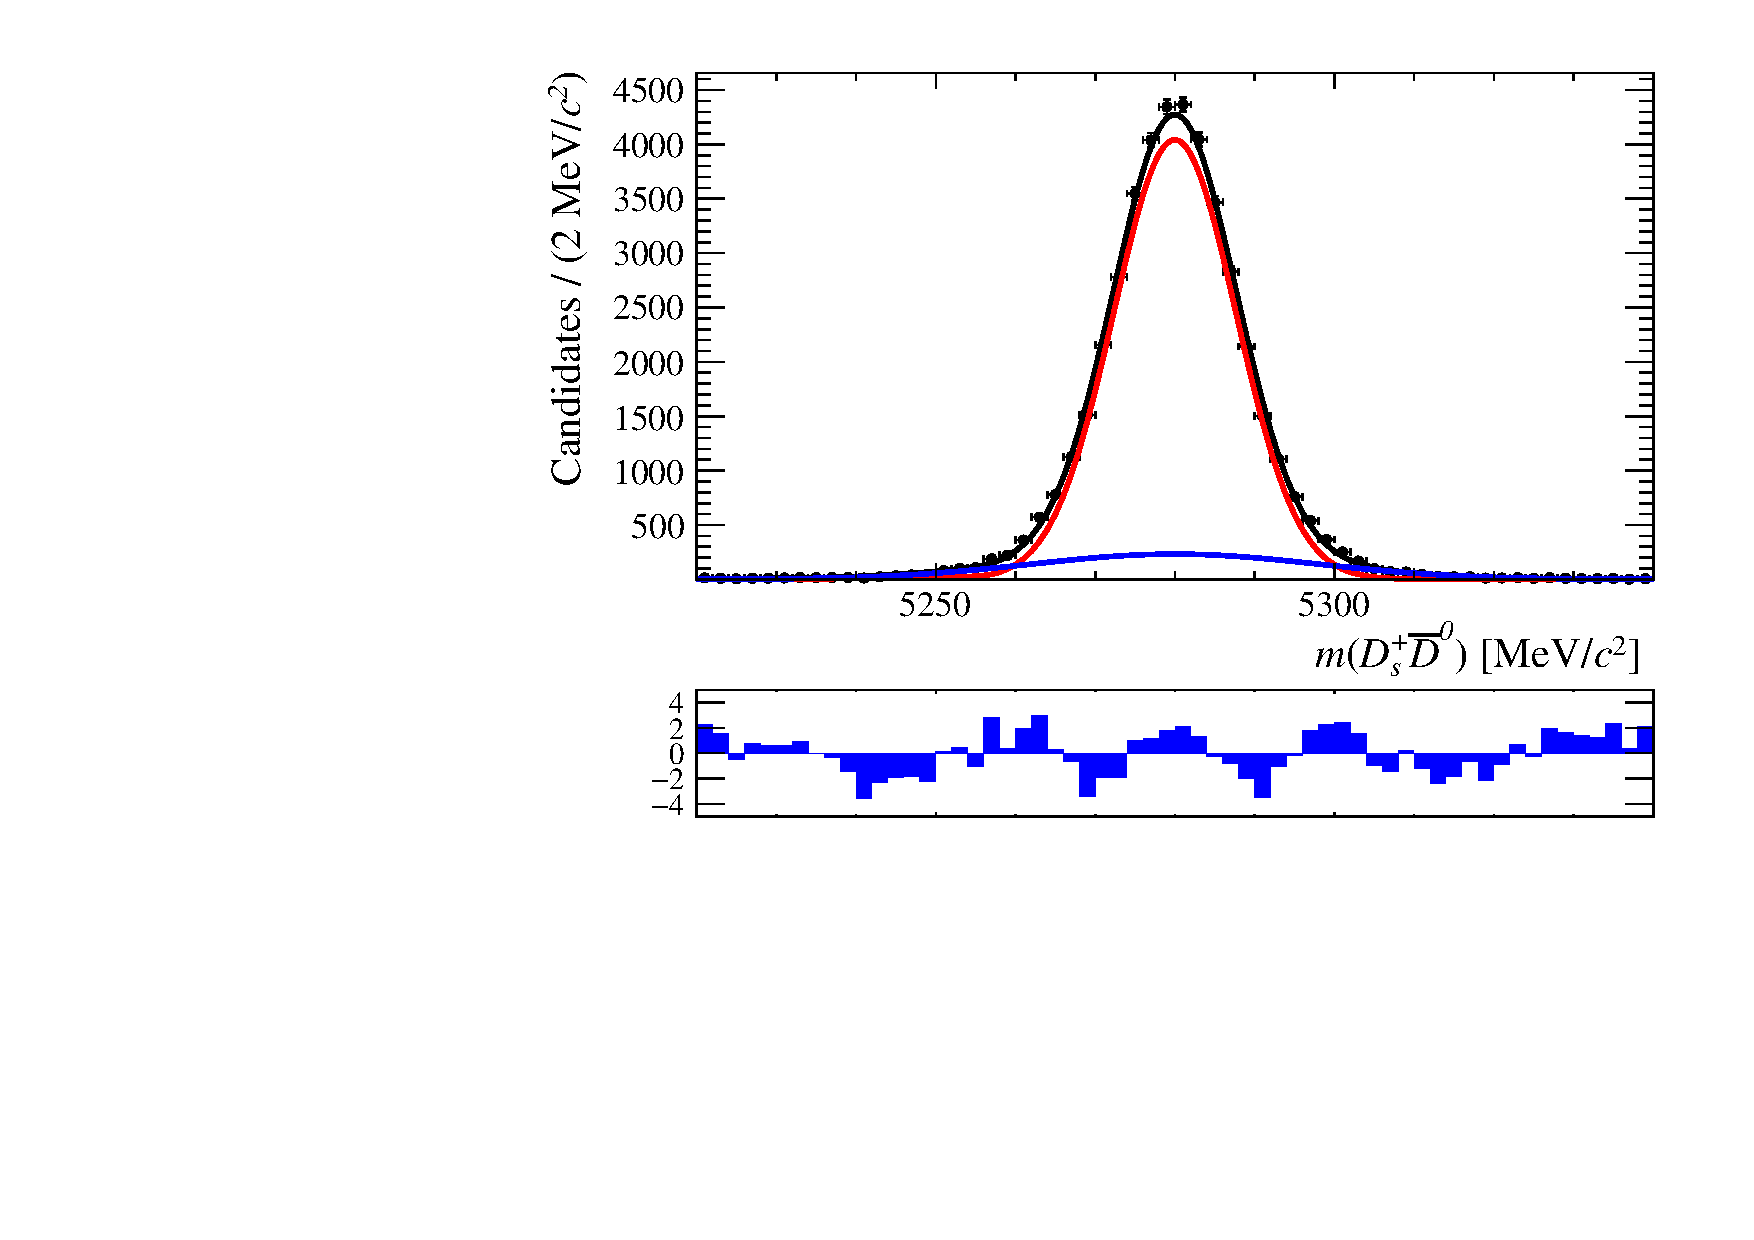
\includegraphics[width=0.40\textwidth]{figs/B2DsPhi/Plot_Signal_Fit_All_B2D0Ds_Ds2KKPi.pdf}
   \caption{\decay{\Dsp}{\Kp\Km\pip}}
   \end{subfigure}\\
   \begin{subfigure}[t]{1.0\textwidth}
      \centering
      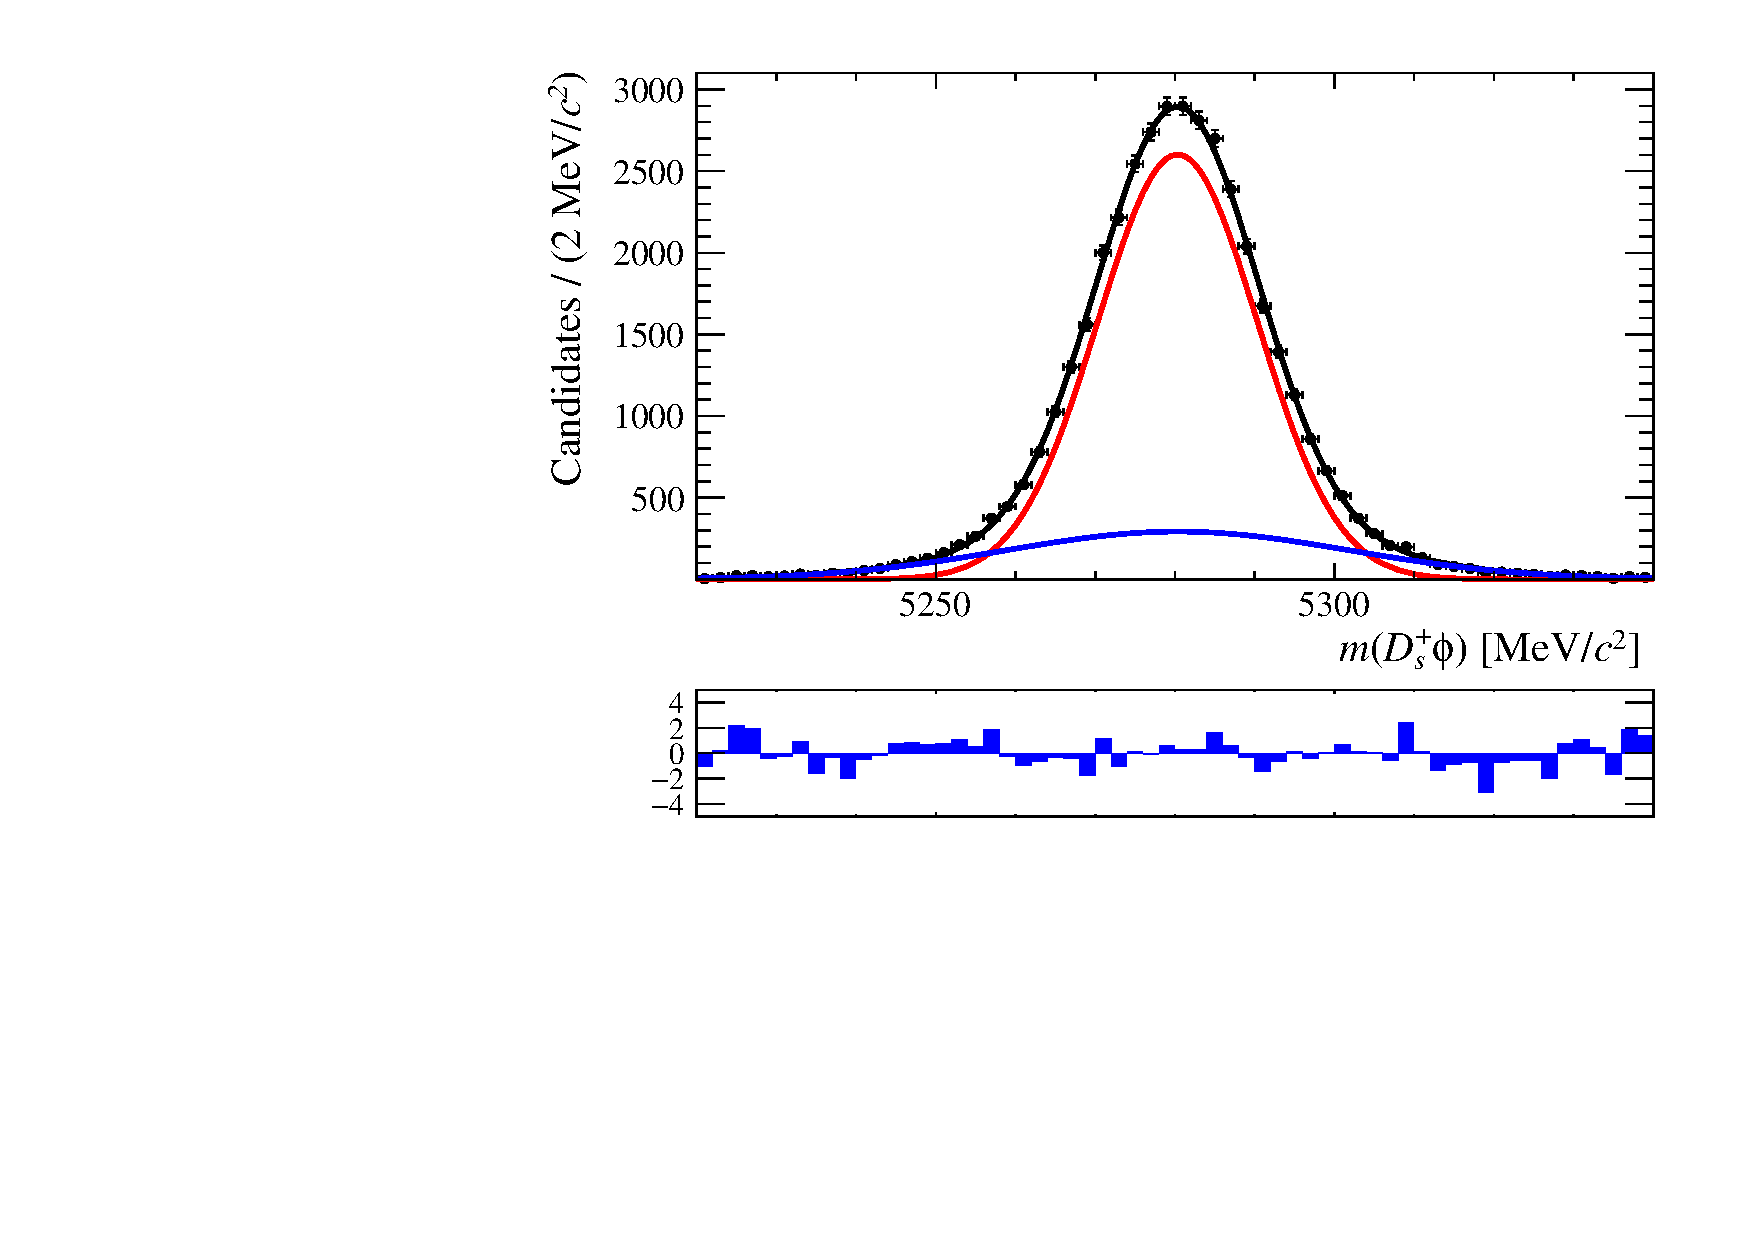
\includegraphics[width=0.40\textwidth]{figs/B2DsPhi/Plot_Signal_Fit_All_B2PhiDs_Ds2PiPiPi.pdf}
      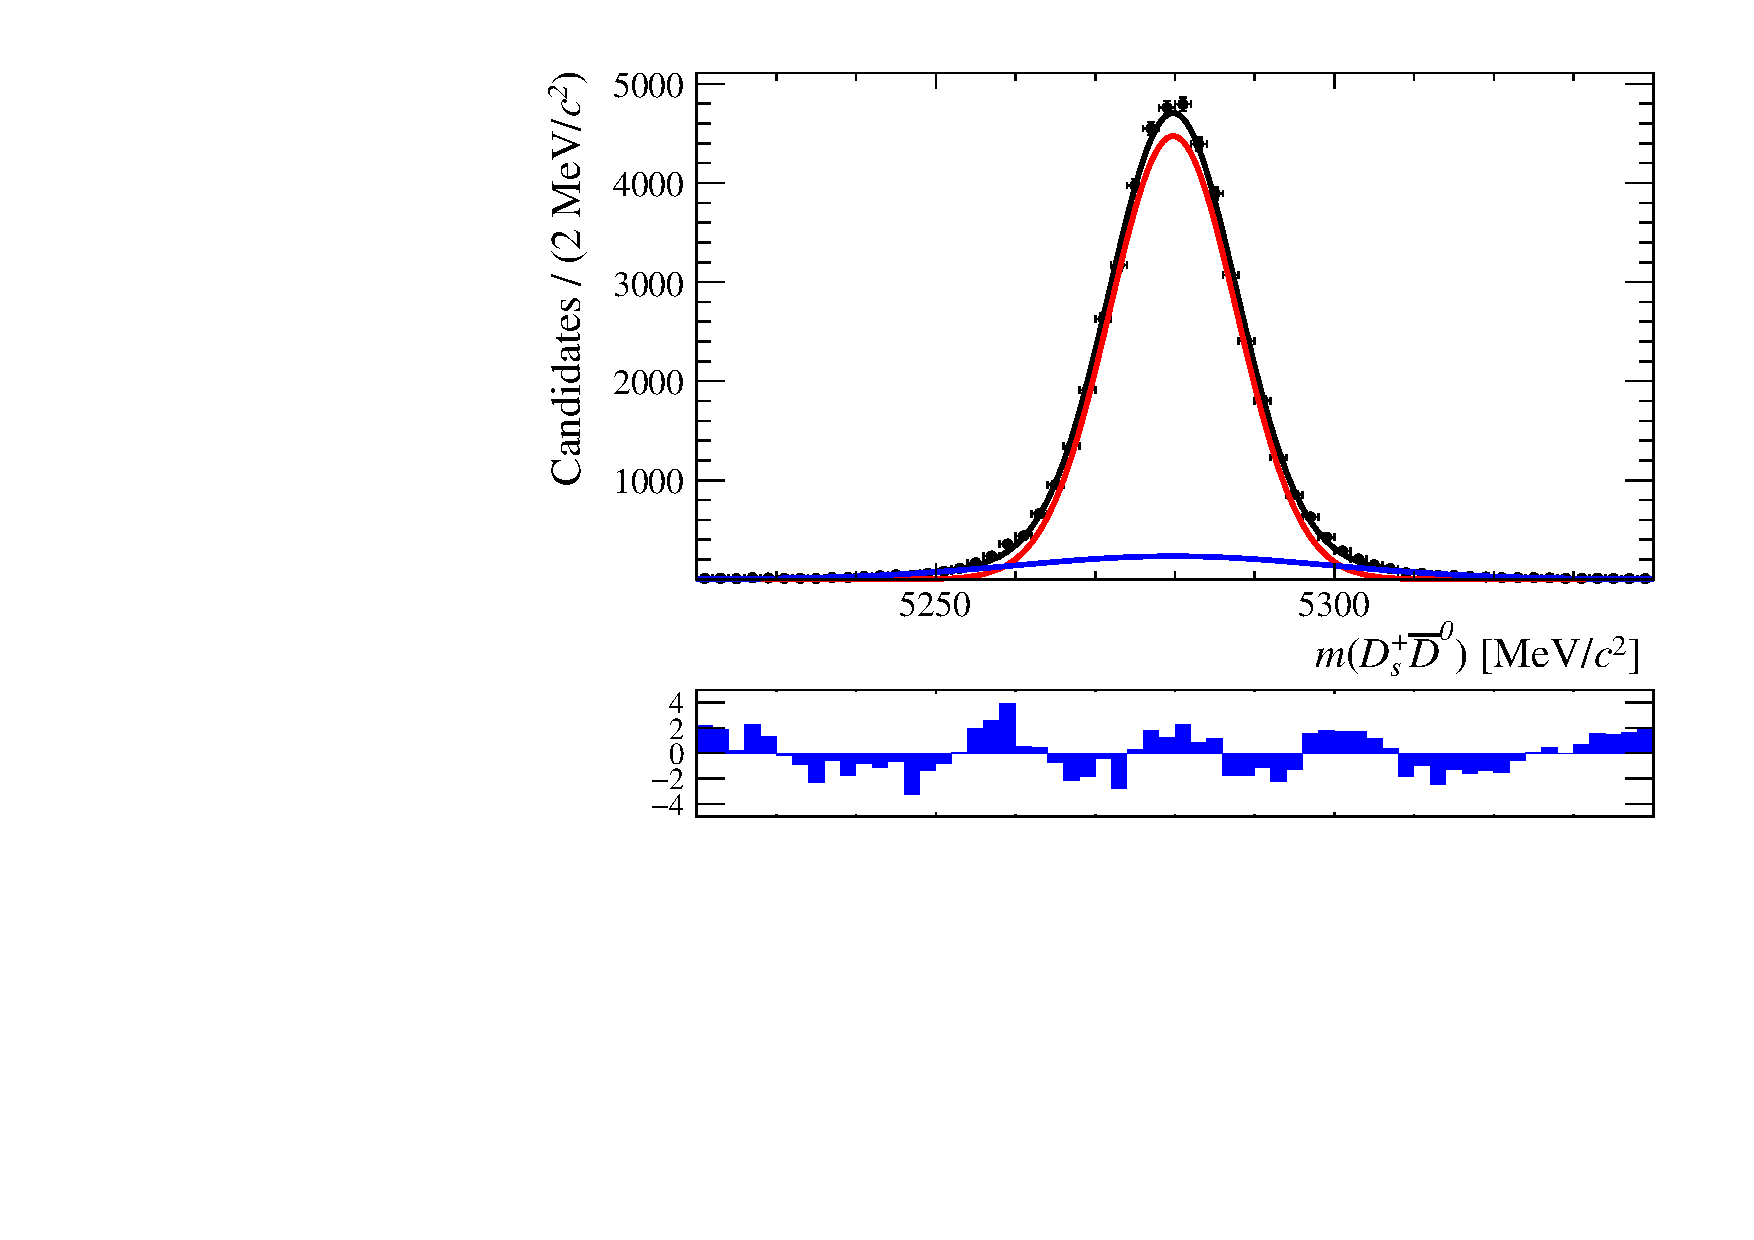
\includegraphics[width=0.40\textwidth]{figs/B2DsPhi/Plot_Signal_Fit_All_B2D0Ds_Ds2PiPiPi.pdf}
      \caption{\decay{\Dsp}{\pip\pim\pip}}
   \end{subfigure}\\
   \begin{subfigure}[t]{1.0\textwidth}
      \centering
      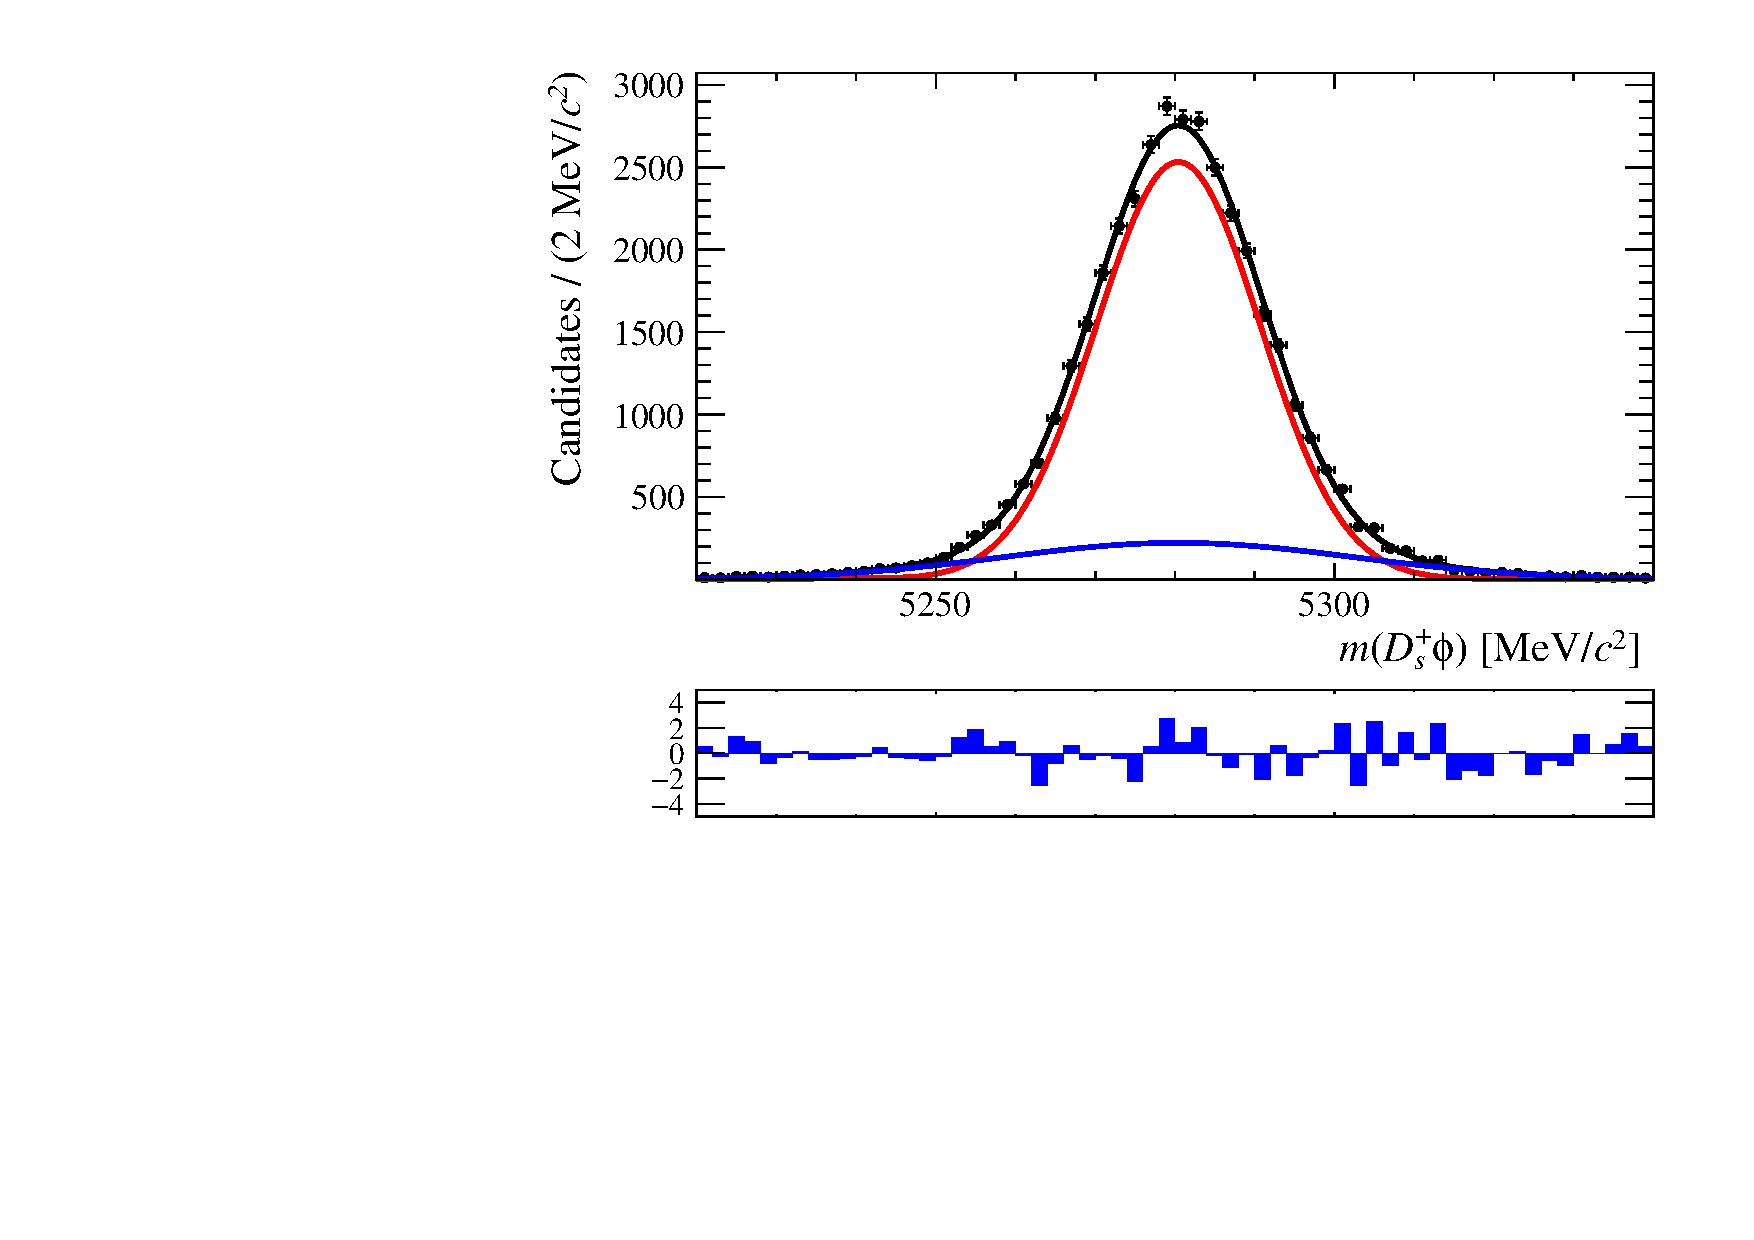
\includegraphics[width=0.40\textwidth]{figs/B2DsPhi/Plot_Signal_Fit_All_B2PhiDs_Ds2KPiPi.pdf}
      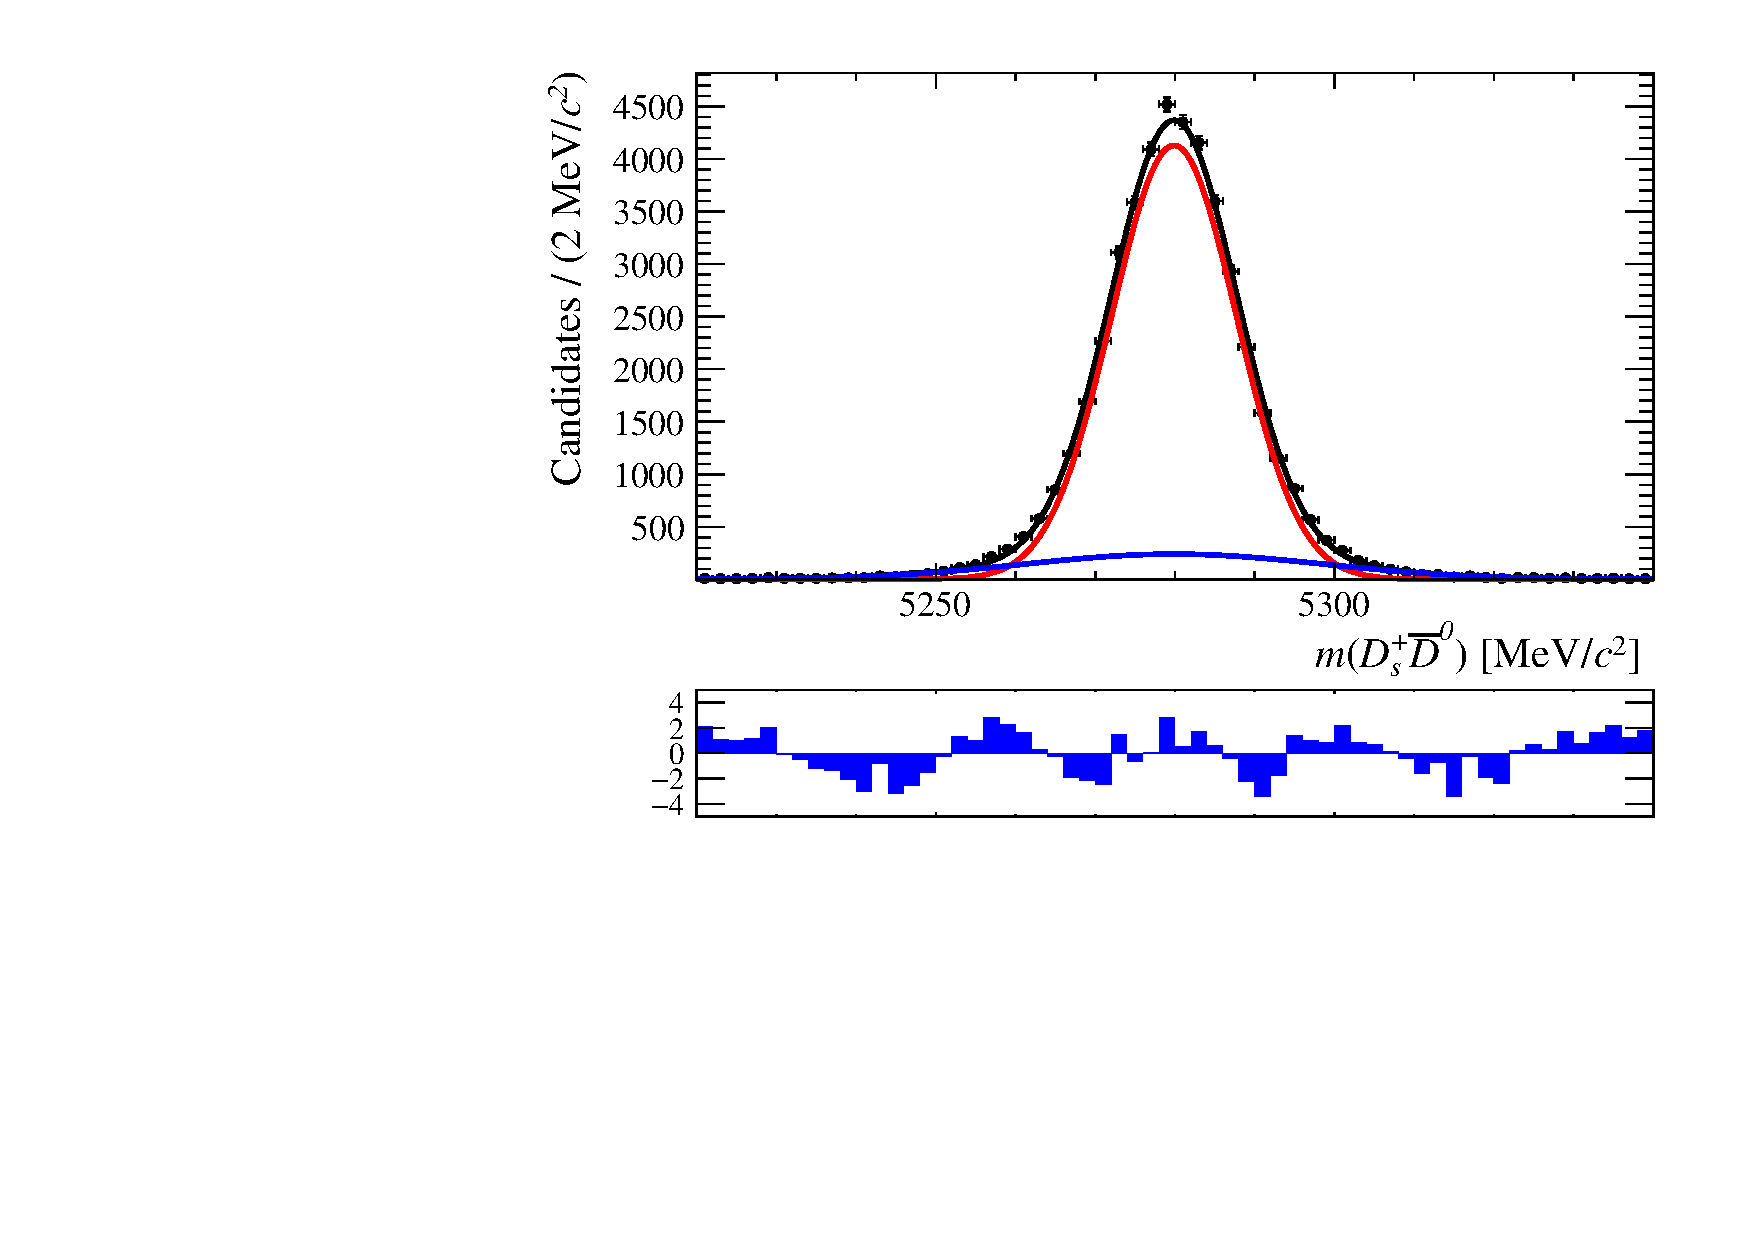
\includegraphics[width=0.40\textwidth]{figs/B2DsPhi/Plot_Signal_Fit_All_B2D0Ds_Ds2KPiPi.pdf}
      \caption{\decay{\Dsp}{\Kp\pim\pip}}
   \end{subfigure}\\
   \caption{Invariant mass fits to simulated signal (left) and normalisation (right) decays. The results of maximum likelihood fits using the signal PDFs are over laid, with the total function in black and the two contributing CB shapes in red and blue.}
   \label{fig:B2DsPhi_signal_fits}   
\end{figure}
%%%%%%%%%%%%%%%%%%%%%%%%%%%%%%%%%%%%%%%%%%%%%%%%%%%%%%%%%%